% Focused revision: original palette/font family retained; numerical details pending later transfer.
% Fig. 1, the teaser: the question, the models under test, the fixed planner with its world-model slot, the task,
% and the four layers along the loop. Drawn at 18 cm, inside \textwidth (18.19 cm). The colours of the model rows
% match Fig. 5 (JEPA blue, W-ar orange, PETS aqua, references grey); the probes are violet.
% The task picture is figures/teaser_task_crop.png, rendered by figures/src/render_scene.py from the flight in Fig. 2,
% oracle_s0_moving100_arena-v0.3.npz (rendered at 2400 x 1000, saved at 1600 x 666; azimuth 135, elevation -12,
% distance 1.45, team-centred, 3.8 s, no paths).
\definecolor{jepa}{HTML}{2A78D6}
\definecolor{war}{HTML}{EB6834}
\definecolor{pets}{HTML}{1BAF7A}
\definecolor{refgrey}{HTML}{8A8984}
\definecolor{ink}{HTML}{0B0B0B}
\definecolor{inktwo}{HTML}{52514E}
\definecolor{rule}{HTML}{D3D1C7}
\definecolor{panel}{HTML}{F7F6F3}
\definecolor{banner}{HTML}{ECEBE7}
\definecolor{probe}{HTML}{6250D6}
\begin{tikzpicture}[
  font=\fontsize{8}{9.2}\selectfont, >={Stealth[length=4pt,width=3.5pt]},
  panel/.style={draw=rule, fill=panel, rounded corners=4pt, line width=0.5pt},
  chip/.style={draw=#1, fill=#1!12, rounded corners=2pt, line width=0.6pt, minimum height=0.42cm,
    text width=3.78cm, font=\fontsize{7}{8}\selectfont, align=left, inner xsep=4pt, inner ysep=1pt, anchor=west},
  stage/.style={draw=inktwo, fill=white, rounded corners=2pt, line width=0.5pt, minimum height=0.5cm,
    text width=3.3cm, align=center},
  slot/.style={draw=ink, dash pattern=on 3pt off 1.5pt, fill=white, rounded corners=2pt, line width=0.9pt,
    minimum height=0.62cm, text width=3.3cm, align=center, font=\fontsize{8}{9.2}\selectfont\bfseries},
  probe/.style={circle, fill=probe, text=white, inner sep=0pt, minimum size=0.36cm, font=\tiny\bfseries},
  flow/.style={->, draw=inktwo, line width=0.6pt},
  real/.style={->, draw=ink, line width=0.9pt},
  heading/.style={font=\fontsize{8}{9.2}\selectfont\bfseries, text=ink, anchor=north west, inner sep=0pt},
  note/.style={font=\fontsize{7.5}{8.6}\selectfont, text=inktwo, inner sep=1pt},
  card/.style={draw=rule, fill=white, rounded corners=3pt, line width=0.5pt},
]
% The question.
\fill[banner, rounded corners=4pt] (0,6.25) rectangle (18,6.85);
\node[font=\small\bfseries, text=ink] at (9,6.55) {Does a model that predicts well also fly well?};

% Left: the models under test.
\draw[panel] (0,2.2) rectangle (4.35,6.05);
\node[heading] at (0.15,5.92) {World models under test};
\node[chip=jepa] at (0.15,5.32) {JEPA: \texttt{full}, \texttt{no\_cross}, \texttt{flat}};
\node[chip=war] at (0.15,4.82) {W-ar: autoregressive state model};
\node[chip=pets] at (0.15,4.32) {PETS: probabilistic ensemble};
\node[note, anchor=west, font=\scriptsize\itshape] at (0.15,3.86) {3 seeds each at 500 and 2,000 episodes};
\node[note, anchor=west] at (0.15,3.44) {references};
\node[chip=refgrey] at (0.15,3.02) {physics; physics + mass estimation};
\node[chip=refgrey] at (0.15,2.52) {oracle U: the true simulator};

% Centre: the planner, fixed for every model, with the world-model slot.
\draw[panel] (4.75,2.2) rectangle (10.9,6.05);
\node[heading] at (4.9,5.92) {Shared planner, fixed (MPPI, 1.5\,s ahead)};
\node[stage] (cand) at (6.9,5.22) {512 candidate plans};
\node[slot] (wm) at (6.9,4.4) {world model under test};
\node[stage] (fut) at (6.9,3.55) {predicted futures};
\node[stage] (pick) at (6.9,2.72) {MPPI-weighted plan};
\draw[flow] (cand) -- (wm);
\draw[flow] (wm) -- (fut);
\draw[flow] (fut) -- (pick);
\draw[->, draw=inktwo, line width=0.9pt] (4.35,4.4) -- (wm.west);
\node[probe] at (9.0,3.55) {1};
\node[probe] at (9.0,4.4) {2};
\node[probe] at (9.0,2.72) {3};

% Right: the task.
\draw[panel] (11.3,2.2) rectangle (18,6.05);
\node[heading] at (11.45,5.92) {Task: three Crazyflie 2 carry a slung load};
\node[anchor=north west, inner sep=0pt] (task) at (11.45,5.62) {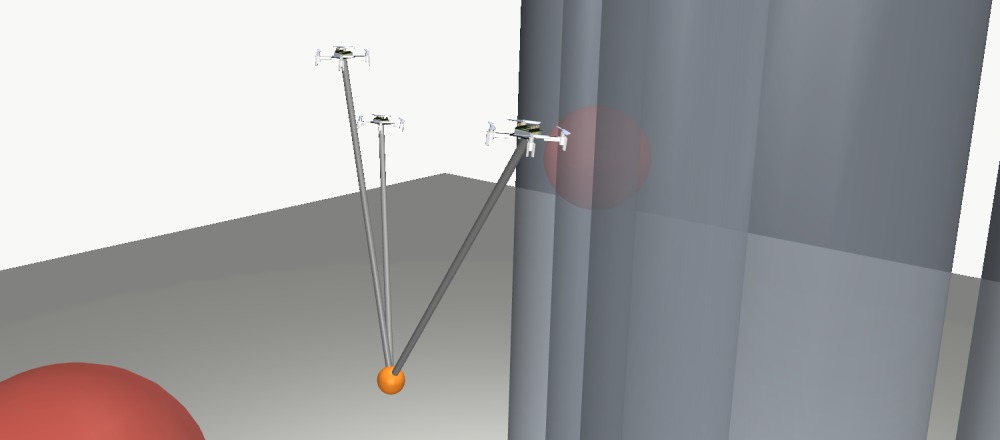
\includegraphics[width=6.4cm]{figures/teaser_task_crop.png}};
\draw[rule, line width=0.5pt] (task.south west) rectangle (task.north east);
\node[probe, draw=white, line width=0.8pt] at ([xshift=-0.3cm,yshift=-0.3cm]task.north east) {4};
\node[chip=refgrey, text width=1.75cm, align=center, anchor=center] at (12.55,2.55) {hidden load mass};
\node[chip=refgrey, text width=1.75cm, align=center, anchor=center] at (14.65,2.55) {0--200\,ms delay};
\node[chip=refgrey, text width=1.75cm, align=center, anchor=center] at (16.75,2.55) {moving obstacles};

% The real loop: the delayed state in, setpoints out.
\draw[real] (11.3,5.22) -- (cand.east);
\node[note, anchor=south, font=\tiny] at (10.05,5.25) {state, 0--200\,ms old};
\draw[real] (pick.south) |- (11.3,2.32);
\node[note, anchor=south, font=\tiny] at (10.05,2.33) {setpoints, 10\,Hz};

% Bottom: the four layers and the test.
\draw[panel] (0,0) rectangle (18,2.0);
\node[heading] at (0.15,1.88) {Four evaluation layers: overview here, definitions in Fig.~4};
\foreach \x/\n/\name/\text in {
    0.15/1/Prediction/{Same plan:\\load trajectory error},
    3.72/2/Counterfactual/{Change one UAV:\\cross-agent effect error},
    7.29/3/Decision/{Regret of the weighted\\execution plan},
    10.86/4/Mission/{Success rate $J$ over\\400 test episodes}} {
  \draw[card] (\x,0.15) rectangle ++(3.42,1.33);
  \node[probe] at (\x+0.28,1.2) {\n};
  \node[anchor=west, font=\fontsize{8}{9.2}\selectfont\bfseries, inner sep=0pt] at (\x+0.52,1.2) {\name};
  \node[anchor=north west, text width=3.10cm, align=left, font=\fontsize{7.5}{8.6}\selectfont, text=inktwo, inner sep=0pt]
    at (\x+0.15,0.95) {\text};
}
% Detailed pictograms are retained and clarified in Fig.4, avoiding duplication.
% The test.
\draw[card, draw=probe, line width=0.8pt] (14.45,0.15) rectangle (17.85,1.48);
\node[anchor=north west, text width=3.1cm, align=left, font=\fontsize{7.5}{8.6}\selectfont, inner sep=0pt] at (14.6,1.37)
  {\textbf{Pre-registered test}\\[1pt]
   {\color{inktwo}Does $L_2$ add information\\about $J$ beyond $L_1$?\\30 learned models.}};
\end{tikzpicture}
